\section{Era computacional}
\label{sec:ubicomp}

	A era dos ~\textit{mainframes} caracterizou-se pela relação de várias pessoas utilizarem um só
	computador, fazendo com que os usuários tivessem uma interação com o computador central
	~\cite{alegomes, passaro}.
	
	Depois surgiram os ~\textit{Personal Computers (PCs)}, em torno de uma época voltada para a
	construção de computadores cada vez menores e mais portáteis. Com isso, uma nova abordagem foi
	criada com a finalidade de ter uma pessoa por computador, tornando o computador como uma ferramenta
	individual de uso.
	
	Com a continuidade da nanotecnologia, cada vez mais novos equipamentos, com maior capacidade de
	processamento e com um tamanho menor, surgiram e impulsionaram o desenvolvimento de diversas
	formas de dispositivos. Na computação ubíqua há vários dispositivos interagindo para oferecer
	recursos para o usuário, ou seja, aqui temos a ideia de vários computadores por pessoa. \\ \\
	
	A tabela ~\ref{tab:eraComputacional} faz o resumo das três eras da computação.
	
	\begin{table} % aqui começa o ambiente tabela
			\centering
			\caption{Eras computacionais propostas por Mark Weiser ~\cite{alegomes}.} % igual ao ambiente
			\begin{tabular}{l|l} 
				\hline % este comando coloca uma linha na tabela
				 Era computacional & Características \\
				\hline
				\hline
				~\textit{Mainframes} & Uma máquina para vários usuários \\
				Computação pessoal & Uma máquina para cada computador \\
				Computação Móvel & Várias máquinas para um usuário \\ 
				\hline
			\end{tabular}
			\label{tab:eraComputacional}
		\end{table}
	
	\subsection{Computação Pervasiva}
	
		A computação pervasiva une uma alta capacidade de comunicação e uma integração com os usuários.
		Aqui já trás a ideia de utilização de informações, obtidas através do contexto, para que o ambiente
		possa integrar a computação, o ambiente e o usuário. Isso é possível devido a troca e utilização de
		serviços entre os dispositivos e o usuário, produzindo assim uma análise do contexto que
		posteriormente poderá ser utilizado para a criação de uma inteligência no ambiente.
	
	\subsection{Computação Móvel}
	
		A computação móvel baseia-se na capacidade de mobilidade dos serviços computacionais. Os
		dispositivos devem oferecer seus recursos, ~\textit{hardware} e ~\textit{software},
		independentemente de suas localizações físicas e seu deslocamento acontece junto com o usuário.
		Nesta tipo de computação são aplicadas diversas tecnologias de comunicação sem fio, tais como,
		~\textit{wifi} e ~\textit{bluetooth}. A exemplo desse tipo de computação temos, atualmente,
		~\textit{notebooks, smartphones, palmtops} e ~\textit{tablets}.

	\subsection{Computação Ubíqua}
	
		Também denominada de ~\textit{ubicomp}, a computação ubíqua une aspectos tanto da
		computação móvel, quanto da computação pervasiva. A ~\textit{ubicomp} possui a finalidade de
		gerar funcionalidades aos usuários a partir de dispositivos presentes no ambiente. Muitos desses
		dispositivos estão presentes em dispositivos caracterizados na computação móvel.
		
		A figura ~\ref{fig:comparativoUbicomp2} exemplifica a combinação de características obtidas a
		partir da computação pervasiva e móvel. A tabela ~\ref{tab:ubicomp} e a figura
		~\ref{fig:comparativoUbicomp} mostram comparativos entre a computação pervasiva, móvel e ubíqua.
		
		% TODO arrumar as citações
		\begin{figure}[h]
			\centering 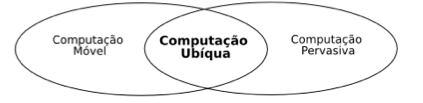
\includegraphics[scale=.75]{figuras/cap2/comparativoUbicomp2.png}
			\caption {\textit{Computação Ubíqua combina características das Computações Móvel e
			Pervasiva ~\cite{alegomes}.}}
			\label{fig:comparativoUbicomp2} 
		\end{figure}
		
		\begin{table} % aqui começa o ambiente tabela 
			\centering
			\caption{Dimensões da Computação Ubíqua ~\cite{passaro}.} % igual ao ambiente figura
			\begin{tabular}{l|c|c|c} 
				\hline % este comando coloca uma linha na tabela
				 & Computação & Computação & Computação \\
				 & Pervasiva & Móvel & Ubíqua \\ 
				\hline
				\hline
				Mobilidade & Baixa	 & Alta & Alta \\
				Imersão computacional & Alta & Baixa & Alta\\
				\hline
			\end{tabular}
			\label{tab:ubicomp}
		\end{table}
		
		\begin{figure}[h]
			\centering 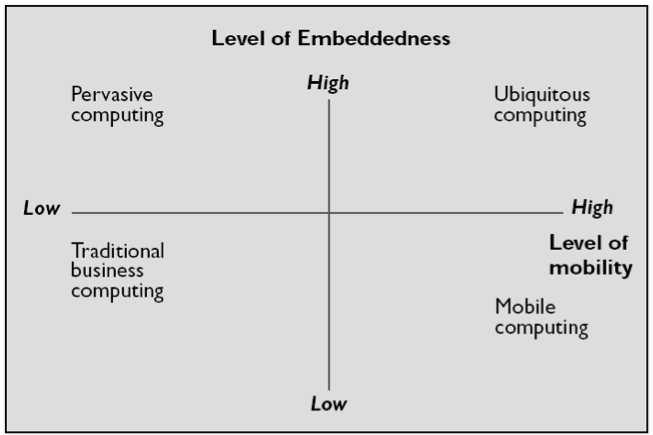
\includegraphics[scale=.45]{figuras/cap2/comparativoUbicomp.png}
			\caption {\textit{Comparativo entre a computação móvel, pervasiva e ubíqua ~\cite{almeida}.}}
			\label{fig:comparativoUbicomp} 
		\end{figure}
		
		Diante disso, a computação ubíqua possui as seguintes propriedades ~\cite{lins}: \\
		
		\begin{enumerate}
		
			\item Invisibilidade \\
			
				Essa é uma característica fundamental na computação ubíqua, algumas vezes o termo ``computação
				invisível'' é utilizado para a ~\textit{ubicomp}. Seus resultados e suas funcionalidades devem
				ocorrer de forma transparente para o usuário, ou seja, é tornar a computação não perceptível no
				foco de atenção do usuário. Isso proporciona que o usuário foque mais nas tarefas e não na parte
				computacional. Através disso a obtenção das informações pertinentes, processamento e obtenção dos
				resultados ocorrem sem que o usuário os solicite a todo o momento, focando principalmente na
				solução da tarefa proposta. \\
			
			%TODO colocar a referência para o Passarinho
	
			\item Pró-atividade \\
			
				Essa característica é definida como a capacidade do sistema em antecipar as intenções do
				usuário. No entanto, é bastante importante que a captura de informações não ocorra de forma
				errônea, para que a mesma não acarrete a uma iniciativa errada. Essas informações podem ser
				analisadas a partir de informações do contexto ao qual o usuário esteja inserido.
				
				Como exemplo de pró-atividade, pode-se citar uma análise hipotética na qual o usuário ao entrar
				na em sua casa, fosse informado se há ou não recados pendentes em sua secretária eletrônica ou
				que seu despertador fosse programável de acordo com sua agenda diariamente. \\
				
			\item Sensibilidade ao contexto \\
			
				Define-se como a interpretação dos diversos dados coletados, a partir dos dispositivos
				distribuídos pelo ambiente inteligente, para que junto com a pró-atividade facilite a antecipação
				de informações e recursos. \\
	
			\item Interfaces naturais \\
		
				Visam principalmente na promoção na usabilidade, procurando enriquecer a capacidade de
				comunicação entre o homem e a máquina, como por exemplo, comandos de voz e comandos gestuais.
				
			
		\end{enumerate} 